\section{Simulation}\label{sec:sim}

	\begin{figure}		
		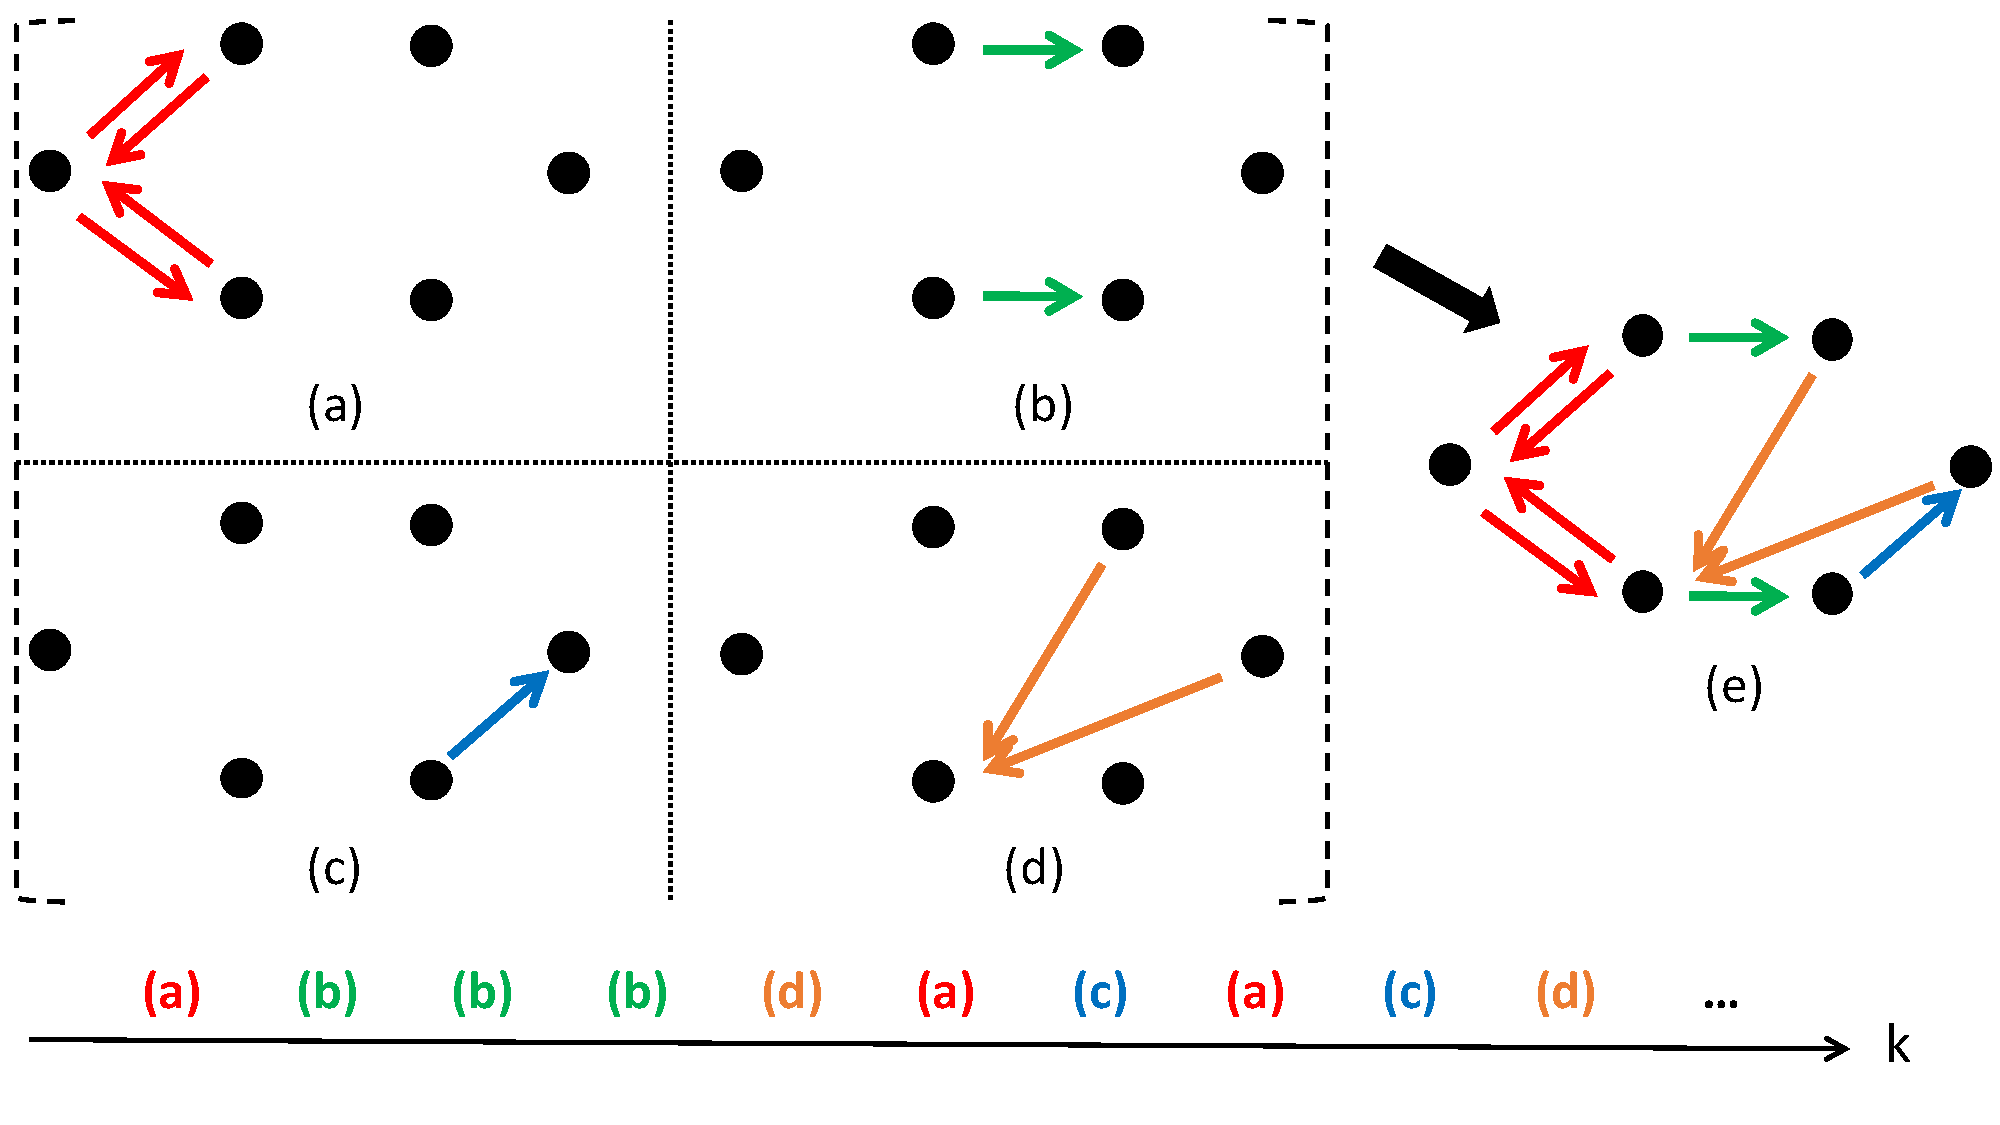
\includegraphics[width=0.5\textwidth]{figures/switch_topo}
		\caption{The dynamically changing interaction topologies used in the simulation: (a)-(d) four types of topologies; (e) the union of these topologies is jointly strongly connected. The bottom axis shows a randomly generated sequence of topologies that satisfy the \fc ness condition.}\label{fig:com_topo}		
	\end{figure}		
			
			
	\begin{figure}%[thpb]
		\centering		
		\begin{subfigure}[b]{0.23\textwidth}
			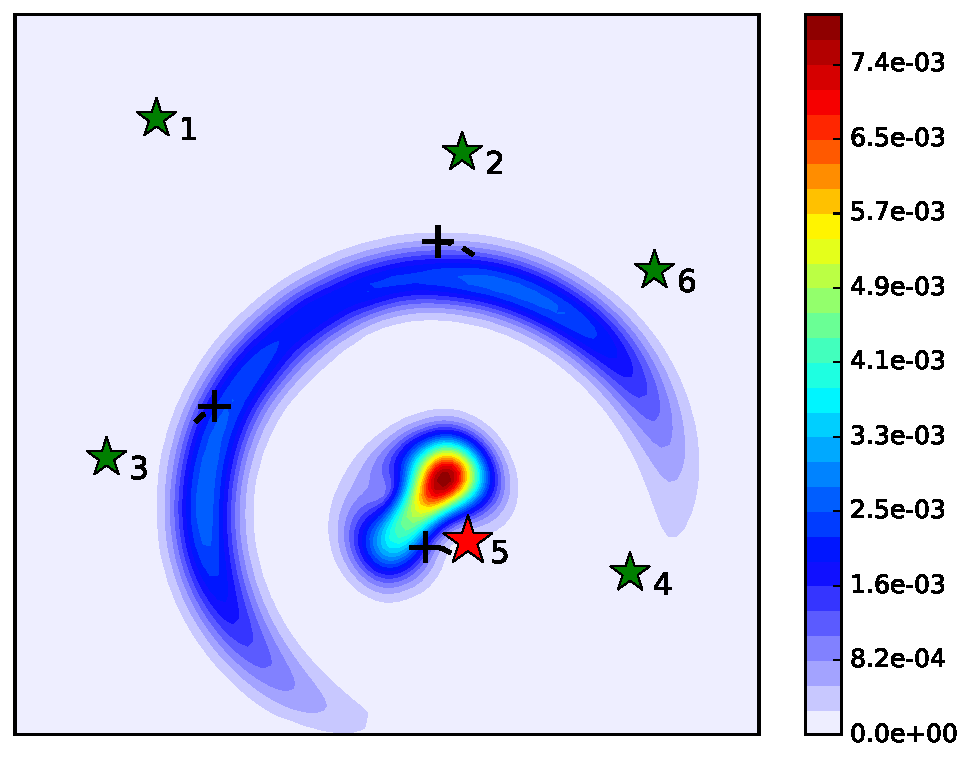
\includegraphics[width=\textwidth]{figures/dbf_hetero_mov_sen_mov_tar_rbt5_step3}
			\caption{\proto-DBF at step 3}\label{fig:step3}
		\end{subfigure}
		\begin{subfigure}[b]{0.23\textwidth}
			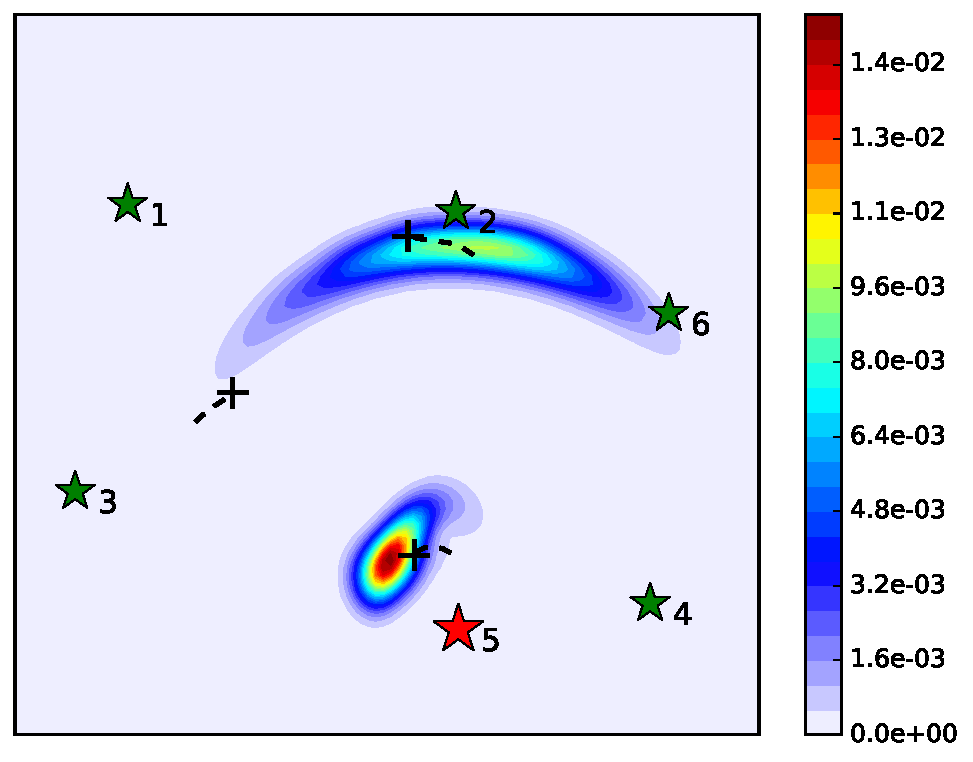
\includegraphics[width=\textwidth]{figures/dbf_hetero_mov_sen_mov_tar_rbt5_step5}
			\caption{\proto-DBF at step 5}\label{fig:step5}
		\end{subfigure}
		\begin{subfigure}[b]{0.23\textwidth}
			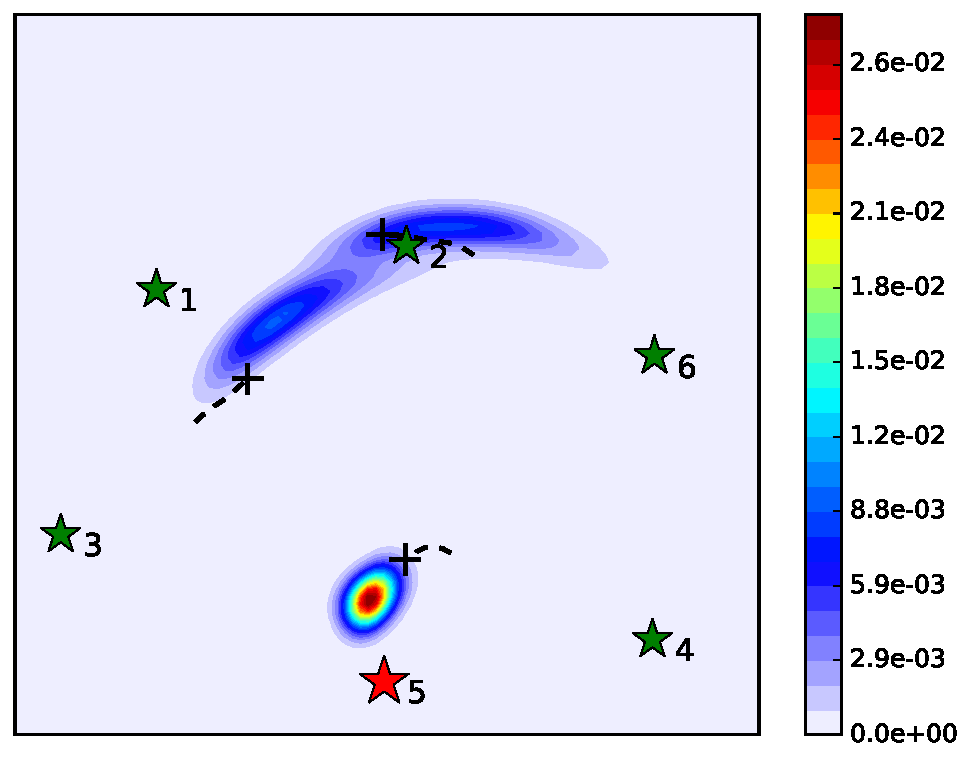
\includegraphics[width=\textwidth]{figures/dbf_hetero_mov_sen_mov_tar_rbt5_step7}
			\caption{\proto-DBF at step 7}\label{fig:step7}
		\end{subfigure}
		\begin{subfigure}[b]{0.23\textwidth}
			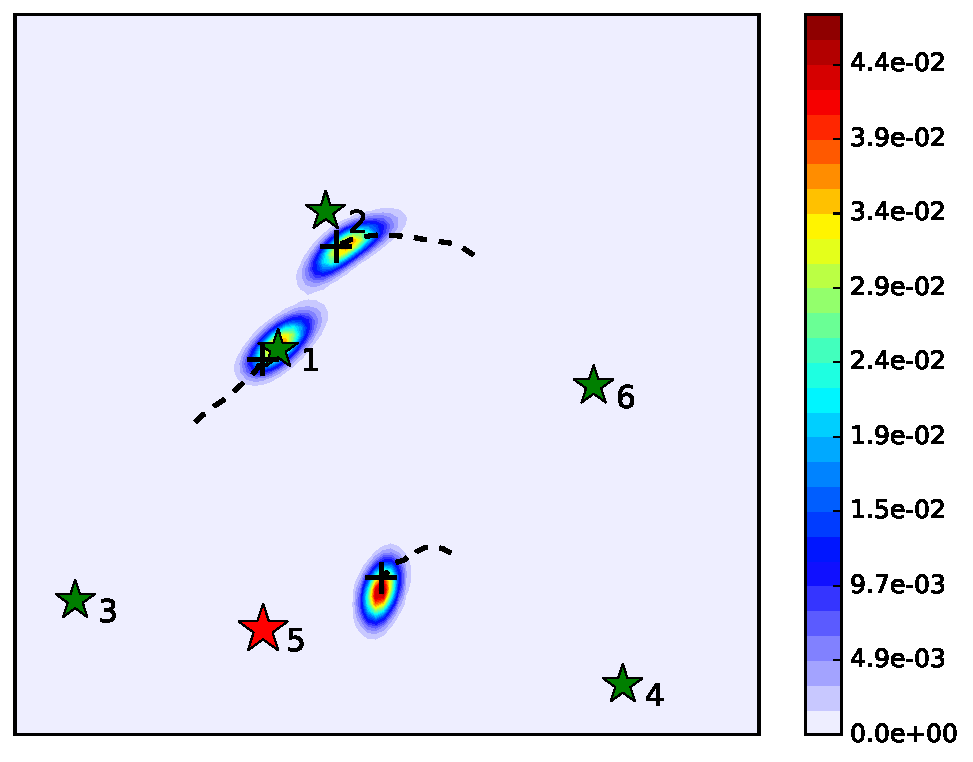
\includegraphics[width=\textwidth]{figures/dbf_hetero_mov_sen_mov_tar_rbt5_step10}
			\caption{\proto-DBF at step 10}\label{fig:step10}
		\end{subfigure}
		\begin{subfigure}[b]{0.23\textwidth}
			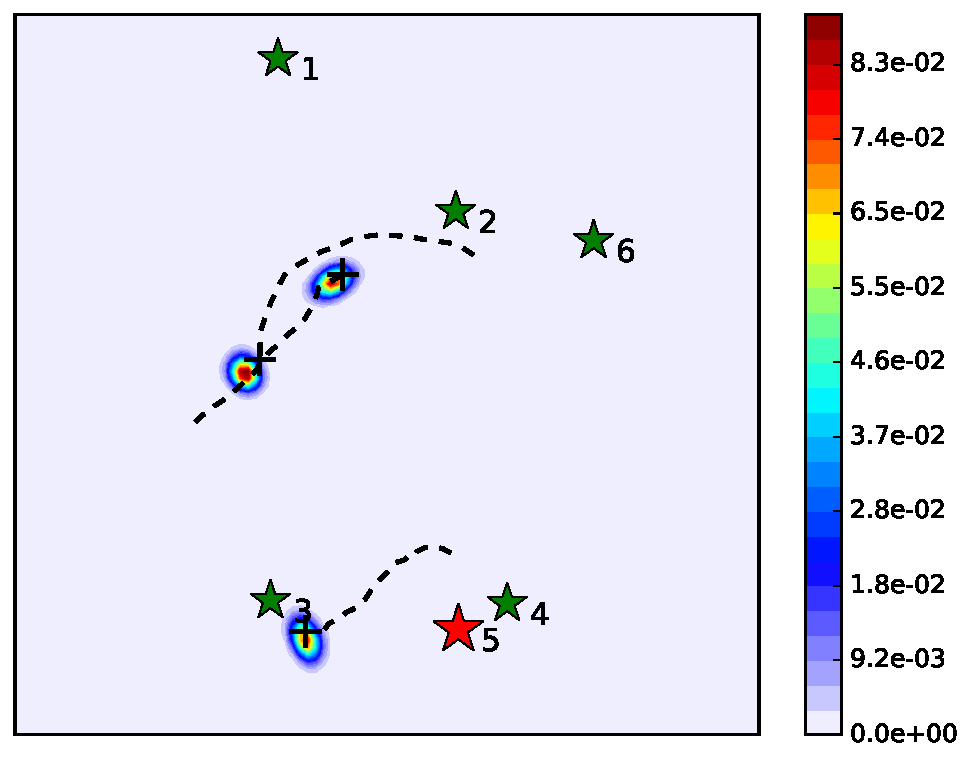
\includegraphics[width=\textwidth]{figures/dbf_hetero_mov_sen_mov_tar_rbt5_step20}
			\caption{\proto-DBF at step 20}\label{fig:step20}
		\end{subfigure}	
		\begin{subfigure}[b]{0.23\textwidth}
			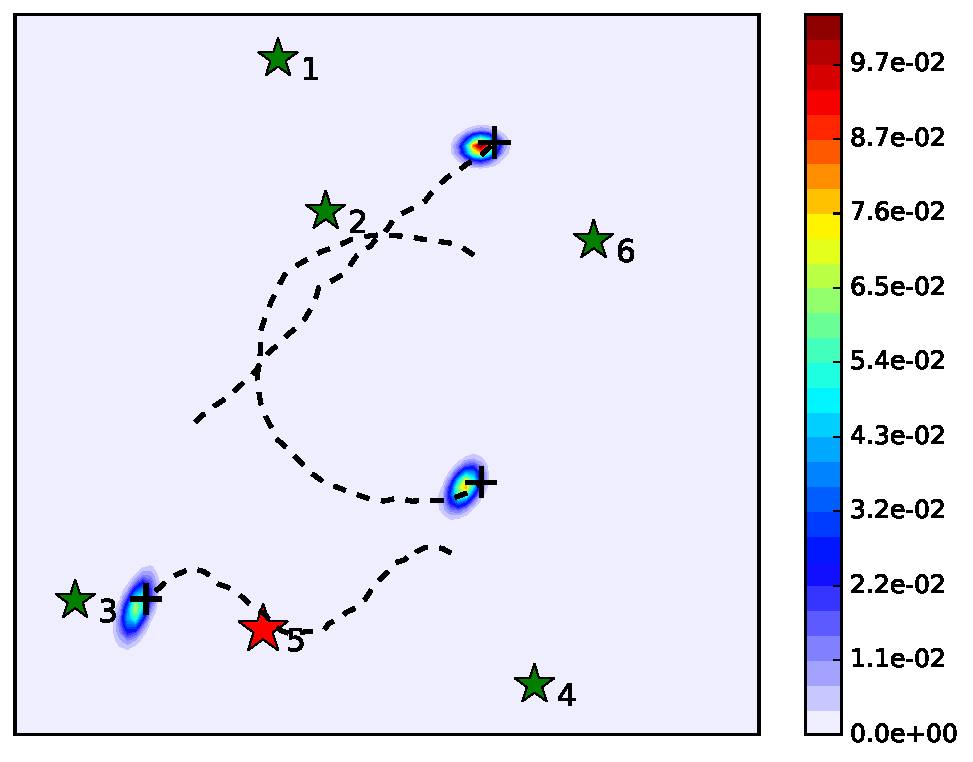
\includegraphics[width=\textwidth]{figures/dbf_hetero_mov_sen_mov_tar_rbt5_step40}
			\caption{\proto-DBF at step 40}\label{fig:step40}
		\end{subfigure}			
		\caption{Evolution of the $1^\text{st}$ UGV's target estimation using \proto-DBF. The colorful background represents the sum of the individual PDF of three targets.}
		%			The uncertainty shrinks as more sensor measurements are utilized.}
		\label{fig:mov_sen_mov_tar1}
		%		\vspace{-1.3em}
	\end{figure}
	
	\begin{figure}%[thpb]
		\centering	
		\begin{subfigure}[b]{0.23\textwidth}
			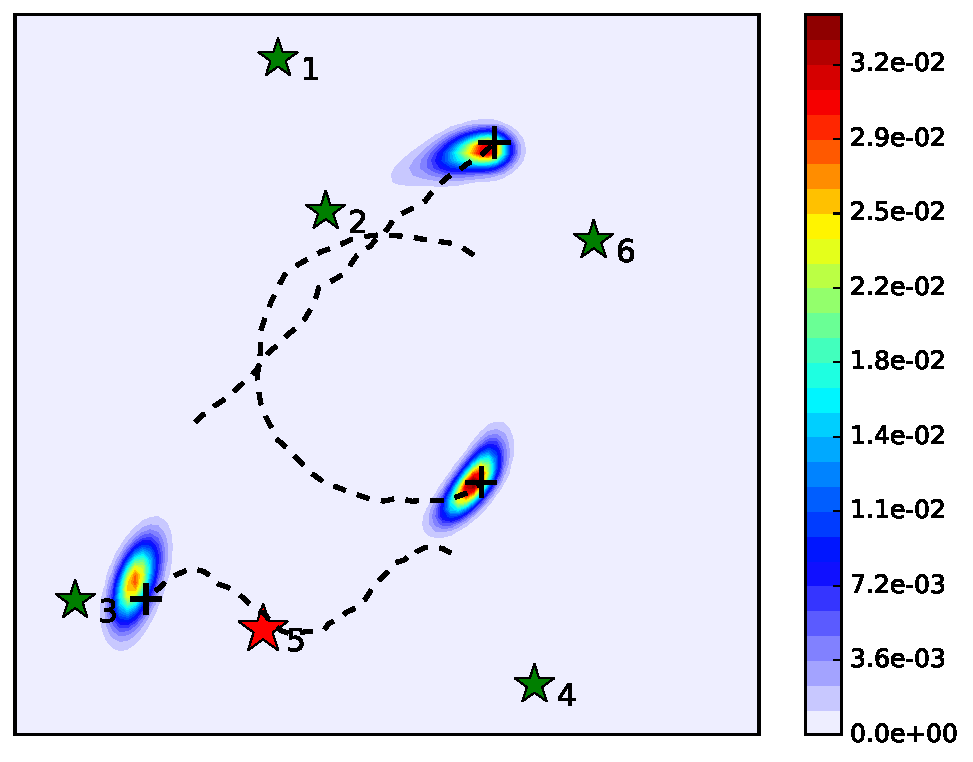
\includegraphics[width=\textwidth]{figures/cons_hetero_mov_sen_mov_tar_rbt5_step40}
			\caption{CbDF at Step 40}\label{fig:cbdf_step40}
		\end{subfigure}	
		\begin{subfigure}[b]{0.23\textwidth}
			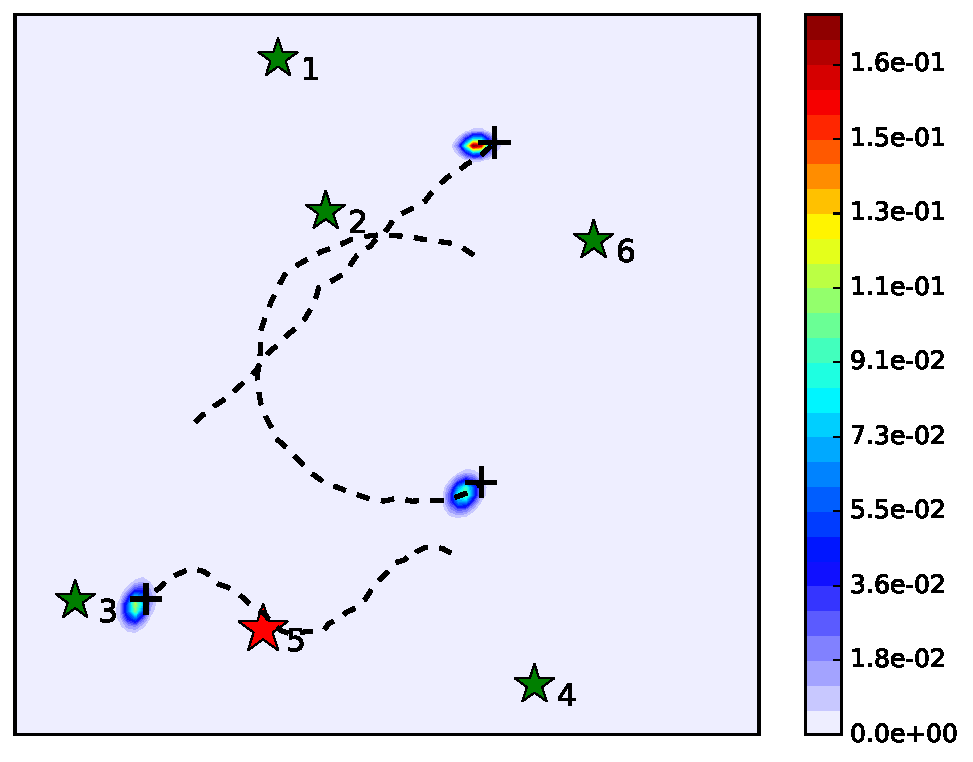
\includegraphics[width=\textwidth]{figures/cent_hetero_mov_sen_mov_tar_rbt1_step40}
			\caption{CF at Step 40}\label{fig:cf_step40}
		\end{subfigure}
		\caption{The $1^\text{st}$ UGV's target estimation using (a) CbDF and (b) CF. The estimation uncertainty remains large for CbDF.}
	\end{figure}


	\begin{figure}%[thpb]
		\centering
		\begin{subfigure}[b]{0.23\textwidth}
			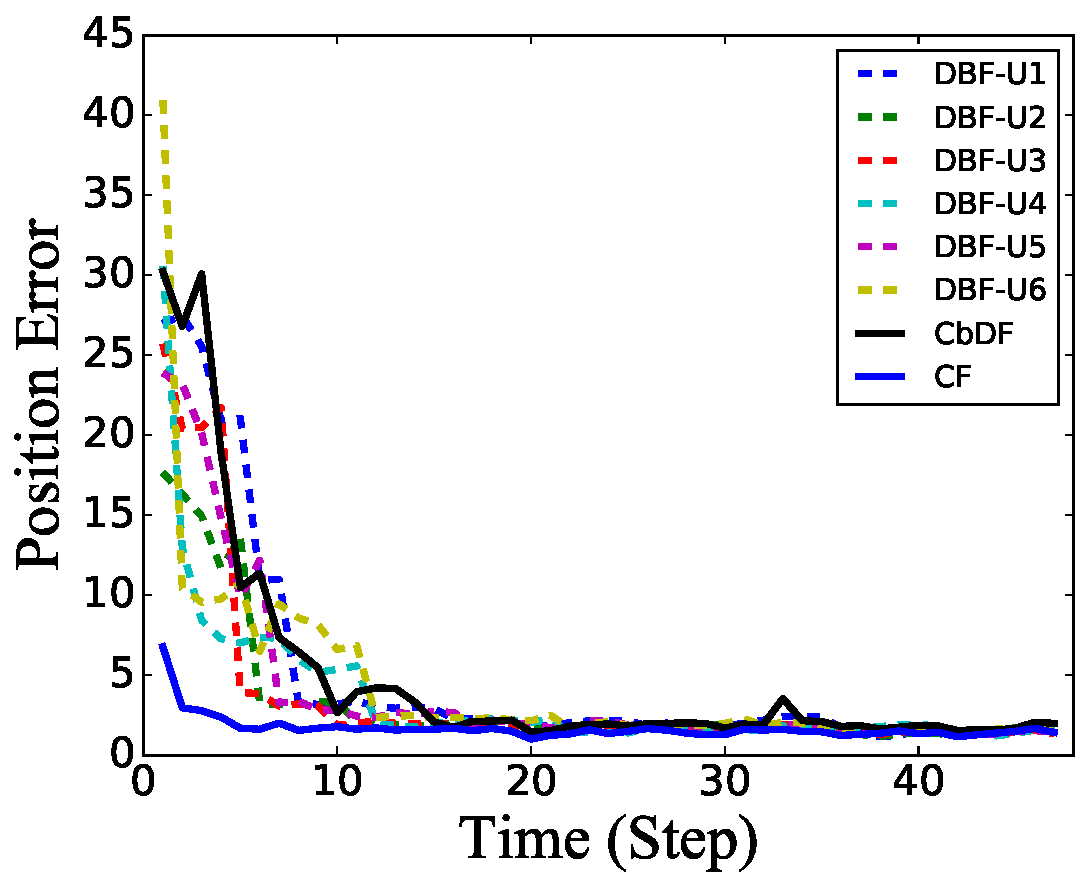
\includegraphics[width=\textwidth]{figures/hetero_mov_sen_mov_tar_pos_err_noise_linear}
			\caption{Position Error of Target $1$}\label{fig:lin_pos_err}
		\end{subfigure}				
		\begin{subfigure}[b]{0.23\textwidth}
			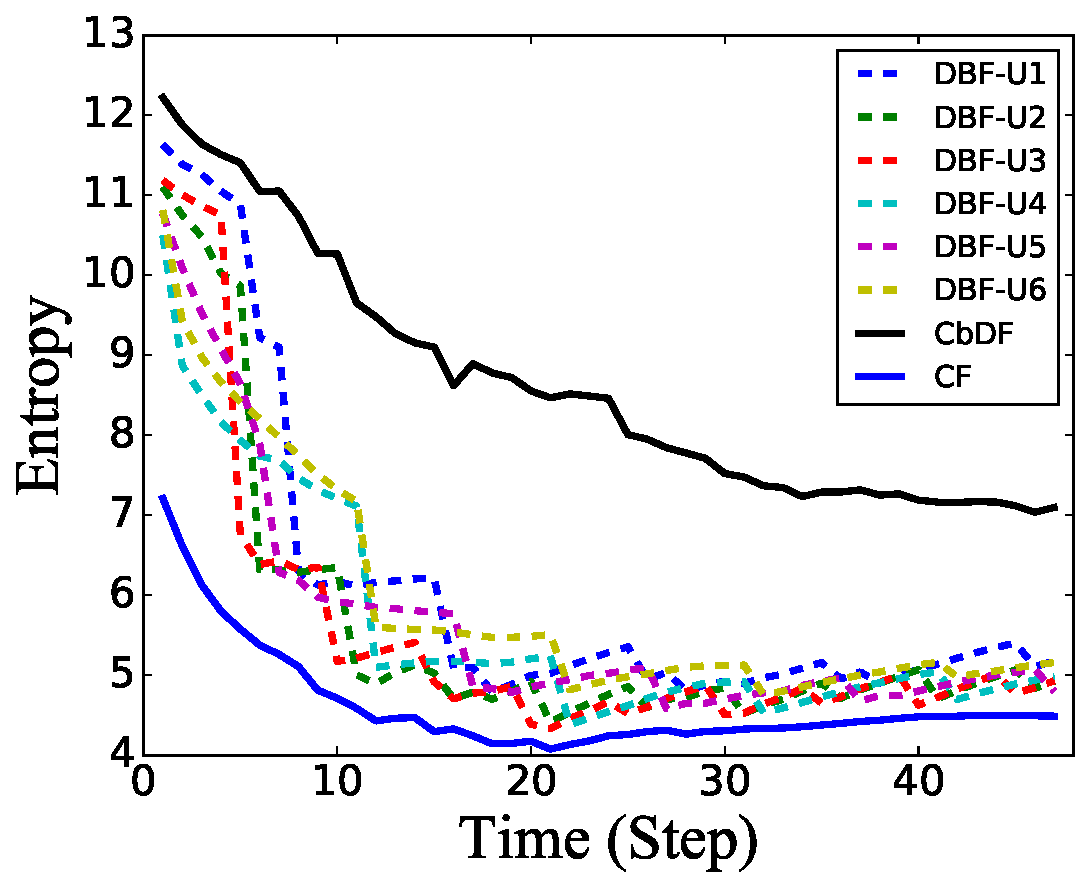
\includegraphics[width=\textwidth]{figures/hetero_mov_sen_mov_tar_entropy_noise_linear}
			\caption{Entropy of Target $1$}\label{fig:lin_ent}
		\end{subfigure}	
		\begin{subfigure}[b]{0.23\textwidth}
			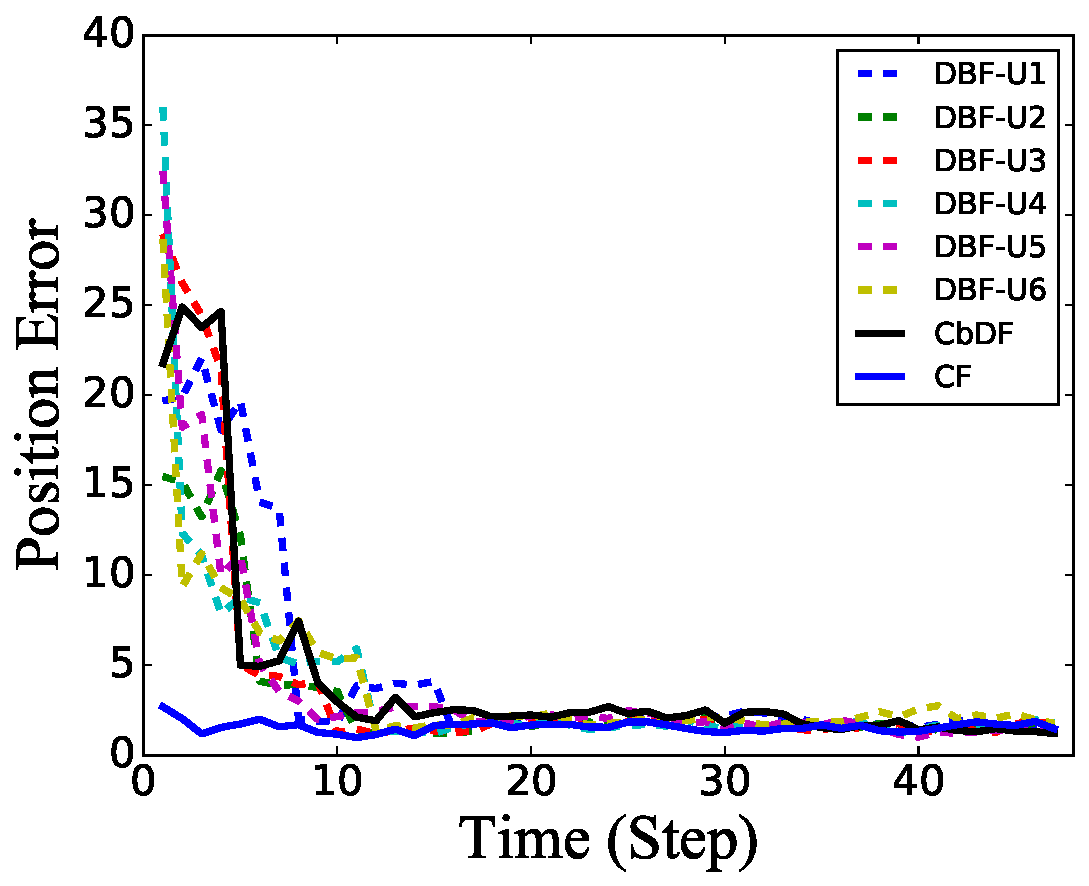
\includegraphics[width=\textwidth]{figures/hetero_mov_sen_mov_tar_pos_err_noise_circle}
			\caption{Position Error of Target $2$}\label{fig:cir_pos_err}
		\end{subfigure}
		\begin{subfigure}[b]{0.23\textwidth}
			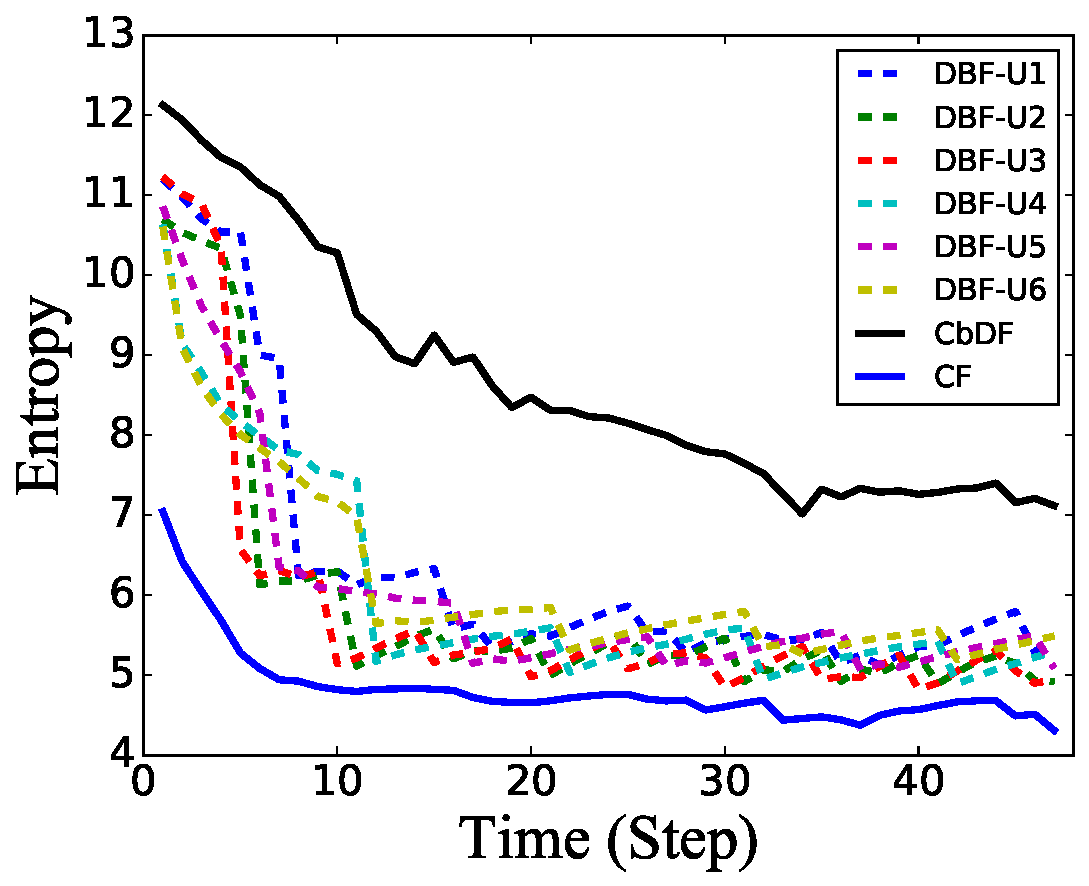
\includegraphics[width=\textwidth]{figures/hetero_mov_sen_mov_tar_entropy_noise_circle}
			\caption{Entropy of Target $2$}\label{fig:cir_ent}
		\end{subfigure}			
		\begin{subfigure}[b]{0.23\textwidth}
			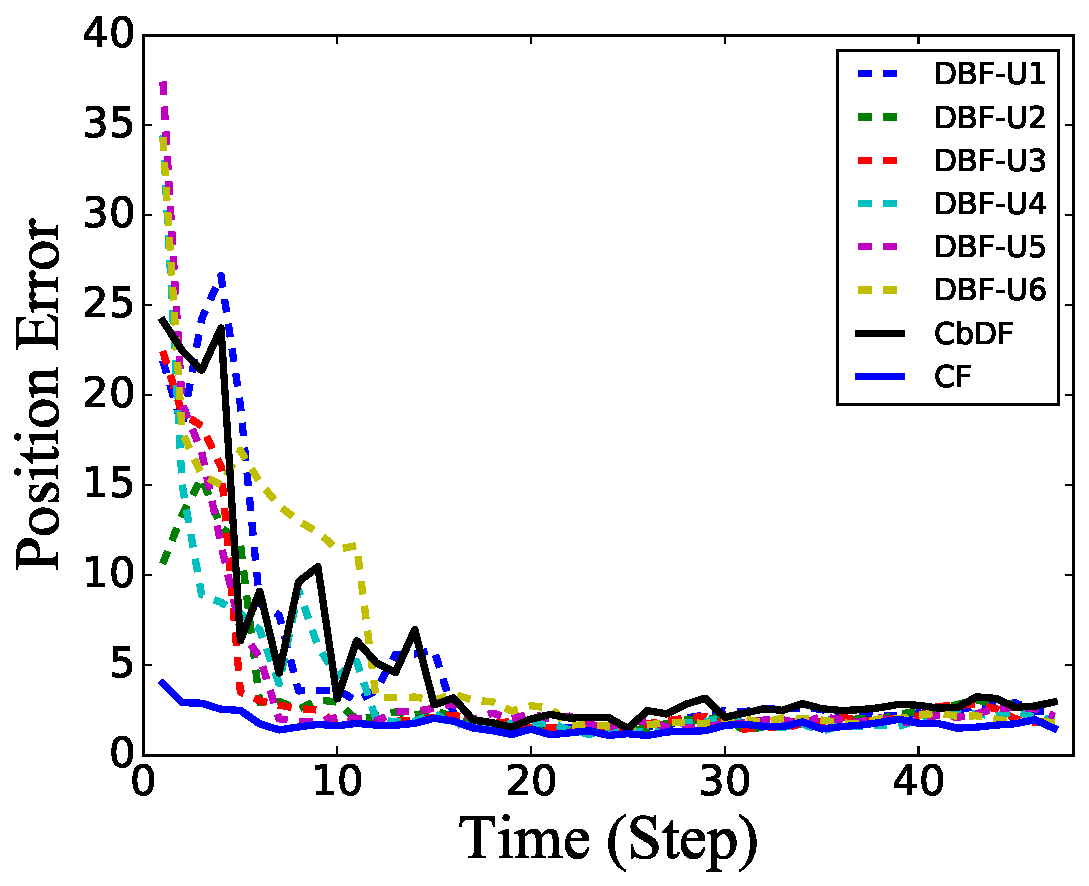
\includegraphics[width=\textwidth]{figures/hetero_mov_sen_mov_tar_pos_err_noise_sin}
			\caption{Position Error of Target $3$}\label{fig:sin_pos_err}
		\end{subfigure}
		\begin{subfigure}[b]{0.23\textwidth}
			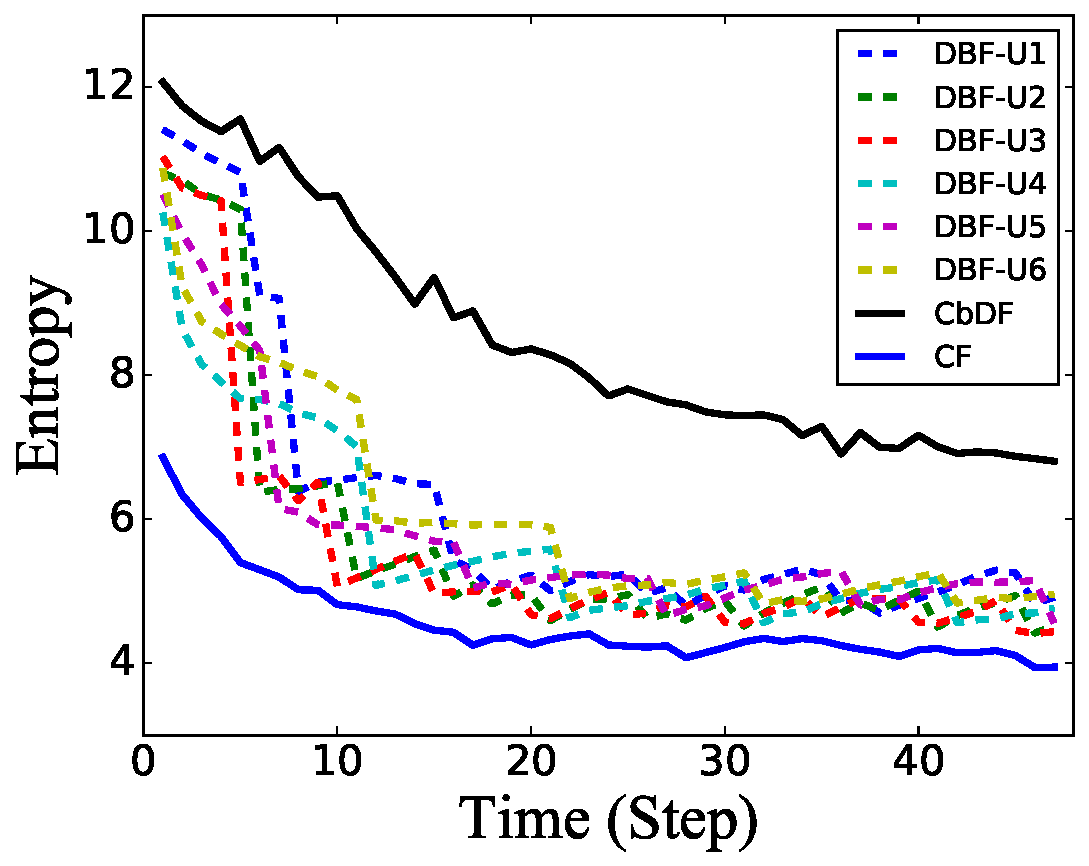
\includegraphics[width=\textwidth]{figures/hetero_mov_sen_mov_tar_entropy_noise_sin}
			\caption{Entropy of Target $3$}\label{fig:sin_ent}
		\end{subfigure}		
		\caption{\textcolor{\revcol}{The average estimation error (a)(c)(e) and the average entropy (b)(d)(f) of ten trials using different filtering approaches. The dotted lines correspond to the results of \proto-DBF by the six UGVs ('U1'-'U6' in the legends).}}
		\label{fig:metrics}
		%		\vspace{-1.3em}
	\end{figure}	

	We conduct a simulation that uses a team of six UGVs to localize three moving targets.
	Every UGV maintains three individual PDFs, each corresponding to a target.
	At each time step, a UGV's sensor can measurement the positions of three targets.
	We assume that the UGVs know the association between the measurement and the corresponding target.
	The targets have different motion models, including the linear motion (target $1$), sinusoidal motion (target $2$), and circular motion (target $3$).
	Three of the UGVs have range-only sensors and the other three UGVs have bearing-only sensors.
	The interaction topology of the UGVs is time-varying and consists of four types, as shown in \cref{fig:com_topo}(a)-(d).
	A randomly generated sequence of topologies is used (\cref{fig:com_topo}f).
	It can be noticed that, the interaction topology is {\fc} when all four types appears repeatedly (\cref{fig:com_topo}e).
	\textcolor{\revcol}{
	Ten test trials are used, with the randomly generated initial positions of UGVs and targets.	
	There exists different methods to implement a Bayesian filter, including the histogram filter and the particle filter \cite{thrun2005probabilistic}. 
	The histogram filter is easy to implement and can keep track of the probability mass over the whole field, but can be computationally heavy for large fields.
	The particle filter, on the contrary, is advantageous when the field is very large, but can introduce inaccuracy due to particle deprivation \cite{thrun2005probabilistic}.
	We use both methods to implement the Bayesian filter in the simulation, and their results are very similar. 
	For the purpose of clarity, we only include the results from the histogram filter here.}
%	Since in this simulation the field is of medium size, we use the histogram filter to implement the Bayesian filter.}
	
	\textcolor{\revcol}{We compare \proto-DBF with two commonly adopted approaches in multi-agent filtering: the consensus-based filter (CbDF) \cite{olfati2006belief} and the centralized filter (CF) \cite{veeravalli2012distributed}. 
	The CbDF requires UGVs to continually exchange their individual PDFs with neighbors, computing the average of its own and the received PDFs. 
	Multiple rounds of communication and averaging are needed at each step to ensure the convergence of UGVs' individual PDFs. 
	The CF assumes a central unit that can constantly receive and fuse all UGVs' latest measurements into a single PDF.}
	
	\cref{fig:mov_sen_mov_tar1} shows the simulation results of a specific trial.
	The sum of the $1^\text{st}$ UGV's individual PDFs are shown in the figures.
	\cref{fig:step3,fig:step5,fig:step7,fig:step10,fig:step20,fig:step40} show that the \proto-DBF can successfully localize and track moving target's positions and effectively reduce the estimation uncertainty, which is similar to the performance of the CF (\cref{fig:cf_step40}).
	On the contrary, CbDF is less effective in reducing the estimation uncertainty (\cref{fig:cbdf_step40}).
	
	We quantitatively compare the three filters in terms of the estimation error and entropy of the uncertainty.
	The estimation error is defined as the difference between the true target position and the MAP estimate of the individual PDF:
	\small\begin{equation*}
		\Delta_k = \|X^\text{MAP}_k-x^g_k\|_2.
	\end{equation*}\normalsize
	The entropy of the uncertainty is
	\small\begin{equation*}
		H_k = \sum\limits_{X_k\in S} -P_{pdf}(X_k)\log(P_{pdf}(X_k)).
	\end{equation*}\normalsize
	The average of the estimation error and entropy of each target across ten trials are shown in \cref{fig:metrics}.
%	For \proto-DBF, we only show the results of the $1^\text{st}$, $3^\text{rd}$, and $5\thi$ UGV for the clarity of the plots.
	It can be noticed that, the CF achieves the most accurate position estimation and fastest entropy reduction. 
	This is an expected result since the CF utilizes all sensor measurements.
	The \proto-DBF achieves similar results as the CF asymptotically. 
	This is a very interesting results, since \proto-DBF only communicates with neighboring UGVs and have a subset of other UGVs' measurements.
	The CbDF achieves similar position estimation performance as the CF and \proto-DBF. 
	However, it fails to effectively reduce the estimation entropy.
	This is because that, the linear combination of PDFs used in the CbDF does not follow the nonlinear nature of Bayesian filtering, thus information is loss during the combination.
	The \proto-DBF, on the other hand, rigorously follows the procedure of Bayesian filtering, and therefore achieves better performance.
	\textcolor{\revcol}{Besides,  CbDF requires multiple rounds of exchanging individual PDFs, which incurs much higher communication burden than \proto-DBF at each time step. 
	Therefore, \proto-DBF is more preferable than CbDF.}
	
	
	
		